\documentclass[10pt]{article}
\usepackage[letterpaper,margin=0.78in]{geometry}
\usepackage{amsmath,amssymb,mathtools}
\usepackage{graphicx}
\usepackage{microtype}
\usepackage{xcolor}
\usepackage[hidelinks]{hyperref}
\usepackage{enumitem}

\definecolor{statusblue}{RGB}{24,77,122}
\setlist{nosep,leftmargin=1.4em}
\setlength{\parindent}{0pt}
\setlength{\parskip}{5pt}

\title{A Literature-Implied Negative Answer to the\\
Unrestricted Isotropic Log-Concave LSI Question}
\author{Run \texttt{fa\_banach\_001} --- review packet}
\date{21 July 2026}

\begin{document}
\maketitle

\noindent\colorbox{statusblue!12}{\parbox{0.95\linewidth}{
\textbf{Status.} \texttt{literature\_implied\_answer (negative)}.
The implication is standard and explicit in later literature; the application
to the source question and the elementary Laplace certificate are recorded
here. No originality is claimed.}}

\section{Source question}

Lee and Vempala ask whether the classical log-Sobolev constant is
$\Theta(1)$ for every isotropic log-concave distribution
\cite[p.~21, immediately before Definition~36]{LeeVempala2018}.
The exact source passage is reproduced below.

\begin{center}

\includegraphics[width=0.98\linewidth]{figures/open_question_crop.png}
\end{center}

In the source convention, after normalizing $\int f^2\,d\mu=1$, a positive
constant means that
\[
  \int |\nabla f|^2\,d\mu \ge c\rho_\mu
  \int f^2\log(f^2)\,d\mu
\]
for some absolute normalization constant $c>0$ and every smooth $f$.

\section{Literature identification}

Bizeul states the standard implication that a classical log-Sobolev
inequality forces all one-dimensional marginals to have subgaussian tails
\cite[p.~1, abstract and (1)--(4)]{Bizeul2026}. Thus any isotropic
log-concave distribution with a non-subgaussian marginal answers the source
question negatively. The supporting passage is reproduced below.

\begin{center}
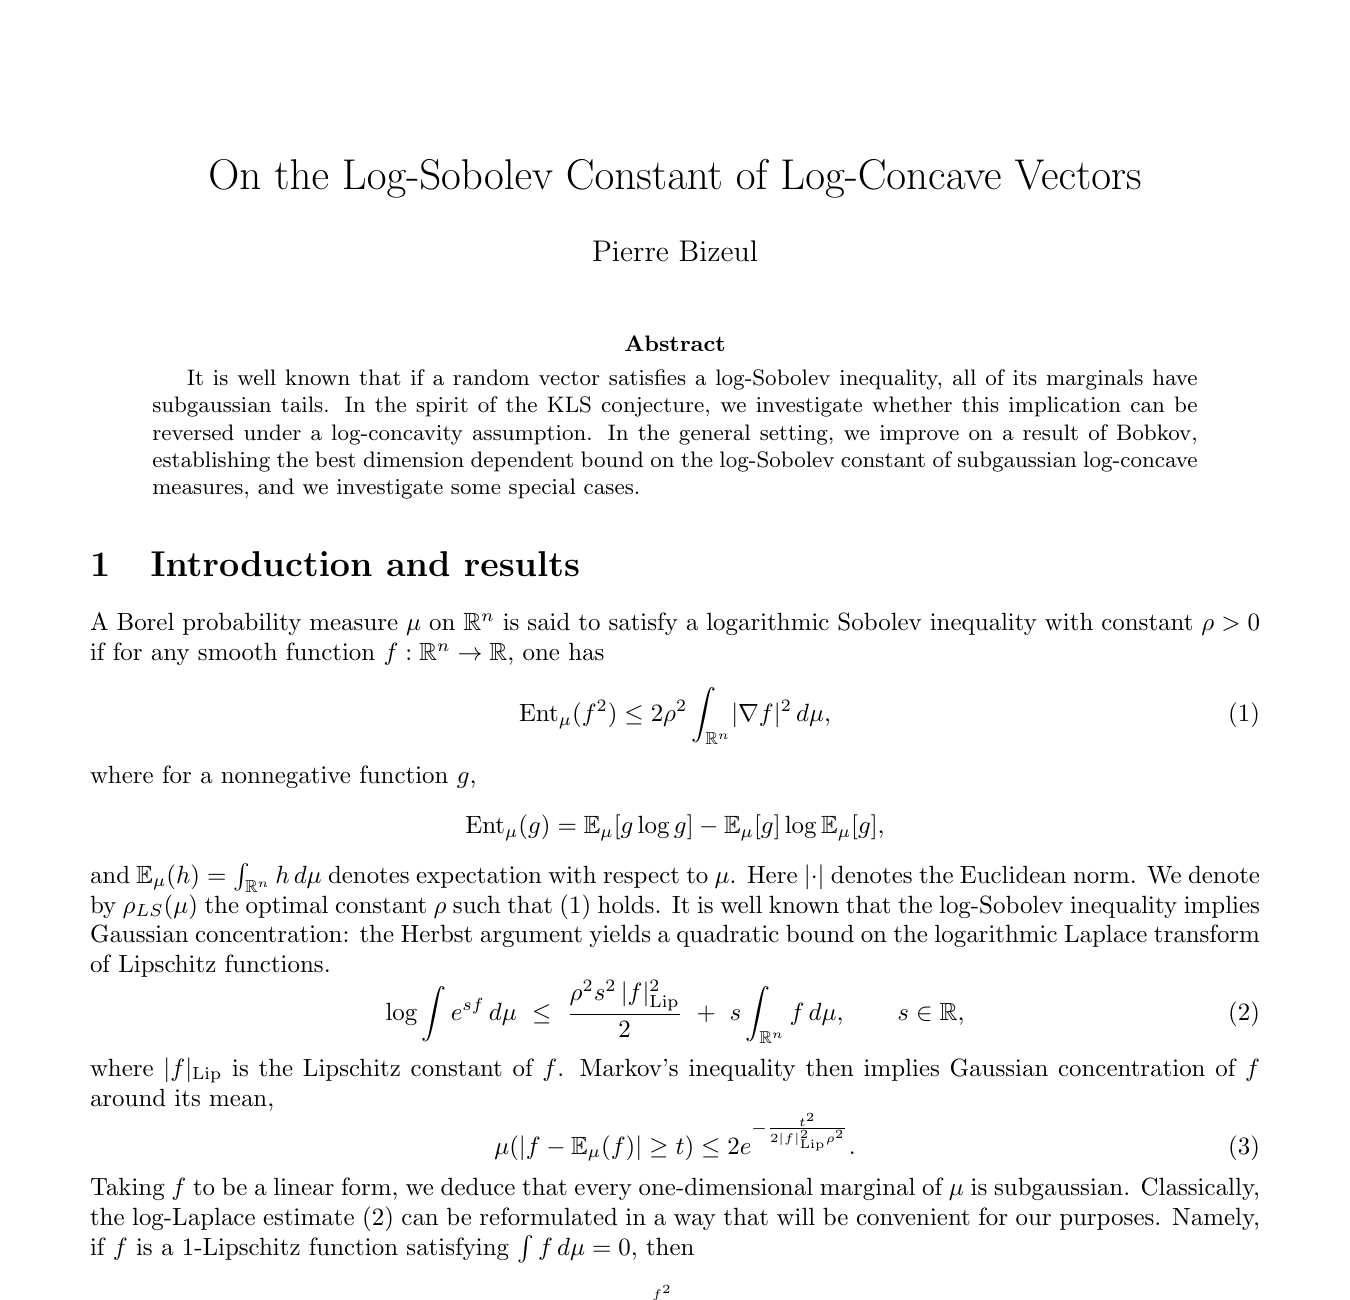
\includegraphics[width=0.98\linewidth]{figures/supporting_implication_crop.png}
\end{center}

The supporting authors do not cite or name the source question. Accordingly,
this is an agent-identified implication, not an explicit claimed resolution in
the literature.

\section{Explicit Laplace certificate}

Let $\alpha=\sqrt2$ and let $\mu$ have density
\[
  p_\alpha(x)=\frac{\alpha}{2}e^{-\alpha|x|},\qquad x\in\mathbb R.
\]
The function $\log p_\alpha$ is concave. Symmetry gives
$\mathbb E_\mu X=0$, and
\[
  \mathbb E_\mu X^2=\frac{2}{\alpha^2}=1,
\]
so $\mu$ is isotropic and log-concave already in dimension one.

For $|s|<\alpha$, its moment-generating function is
\[
  M(s)=\mathbb E_\mu e^{sX}=\frac{\alpha^2}{\alpha^2-s^2}.
\]
Fix $0<t<\alpha/2$ and define the smooth normalized function
\[
  f_t(x)=\frac{e^{tx}}{\sqrt{M(2t)}}.
\]
Then $\int f_t^2\,d\mu=1$ and
\[
  \int |f_t'|^2\,d\mu=t^2.
\]
On the other hand,
\begin{align*}
  \operatorname{Ent}_\mu(f_t^2)
  &=\int f_t^2\log(f_t^2)\,d\mu \\
  &=2t\frac{M'(2t)}{M(2t)}-\log M(2t) \\
  &=\frac{8t^2}{\alpha^2-4t^2}
    -\log\!\left(\frac{\alpha^2}{\alpha^2-4t^2}\right).
\end{align*}
As $t\uparrow\alpha/2$, this entropy tends to $+\infty$, while the
Dirichlet energy tends to $\alpha^2/4=1/2$. Consequently
\[
  \inf_f
  \frac{\int |f'|^2\,d\mu}{\operatorname{Ent}_\mu(f^2)}=0,
\]
and the source-normalized log-Sobolev constant is exactly zero. This proves
the negative answer without invoking the general concentration implication.

\section{Scope, search bounds, and review verdict}

The conclusion applies to the unrestricted wording only. It does not
contradict the bounded-support estimate in the source, nor does it decide
dimension-free LSI bounds under a subgaussian-tail assumption.

The bounded novelty/status search covered the run's registry, solution,
attempt, and proof-gap indexes; exact-title and exact-phrase searches; and
arXiv:1712.01791 and arXiv:2306.12997. No source was found that explicitly
claims to answer the Lee--Vempala question. Since arXiv:2306.12997 records the
decisive standard implication, the correct classification is
\emph{literature-implied answer}, not an original counterexample.

\textbf{Human-review recommendation.} Accept the negative implication and
the elementary certificate. Preserve the scoped literature-implied status.

\begin{thebibliography}{9}
\bibitem{LeeVempala2018}
Y.~T. Lee and S.~S. Vempala,
\emph{The Kannan--Lov\'asz--Simonovits Conjecture},
arXiv:1807.03465 (2018).

\bibitem{Bizeul2026}
P.~Bizeul,
\emph{On the Log-Sobolev Constant of Log-Concave Vectors},
arXiv:2306.12997v3 (2026), accepted in the Journal of Functional Analysis.
\end{thebibliography}

\end{document}

